\chapter{Event Organizer Rules}

\section{Venue}

Hockey should be played in a gym that is large enough to house the playing field.
The surface should be smooth to protect stick blades while still allowing traction for tires.
Indoor court surfaces that provide some absorption of falls such as sprung floors are ideal to reduce injuries.

\section{Officials}

The host must designate the following officials for each hockey tournament:
\begin{itemize}
\item Hockey Director
\item Board of Referees
\end{itemize}

\begin{comment2016}

\section{Communication}

\section{Age Groups}

\section{Practice}

\end{comment2016}

\section{Playing Field}

\subsection{Dimensions}

% Definiere eine Funktion zum Zeichnen eines Rechtecks
\newcommand{\drawRectangle}[4]{
	\def\xcenter{#1} % x-Koordinate des Mittelpunkts
	\def\ycenter{#2} % y-Koordinate des Mittelpunkts
	\def\width{#3}   % Breite des Rechtecks
	\def\height{#4}  % Höhe des Rechtecks
	
	% Berechne die Ecken des Rechtecks
	\def\xmin{\xcenter - \width/2}
	\def\xmax{\xcenter + \width/2}
	\def\ymin{\ycenter - \height/2}
	\def\ymax{\ycenter + \height/2}
	
	% Zeichne das Rechteck
	\fill[orange] (\xmin, \ymin) rectangle (\xmax, \ymax);
}

\setlength{\unitlength}{0.1mm}
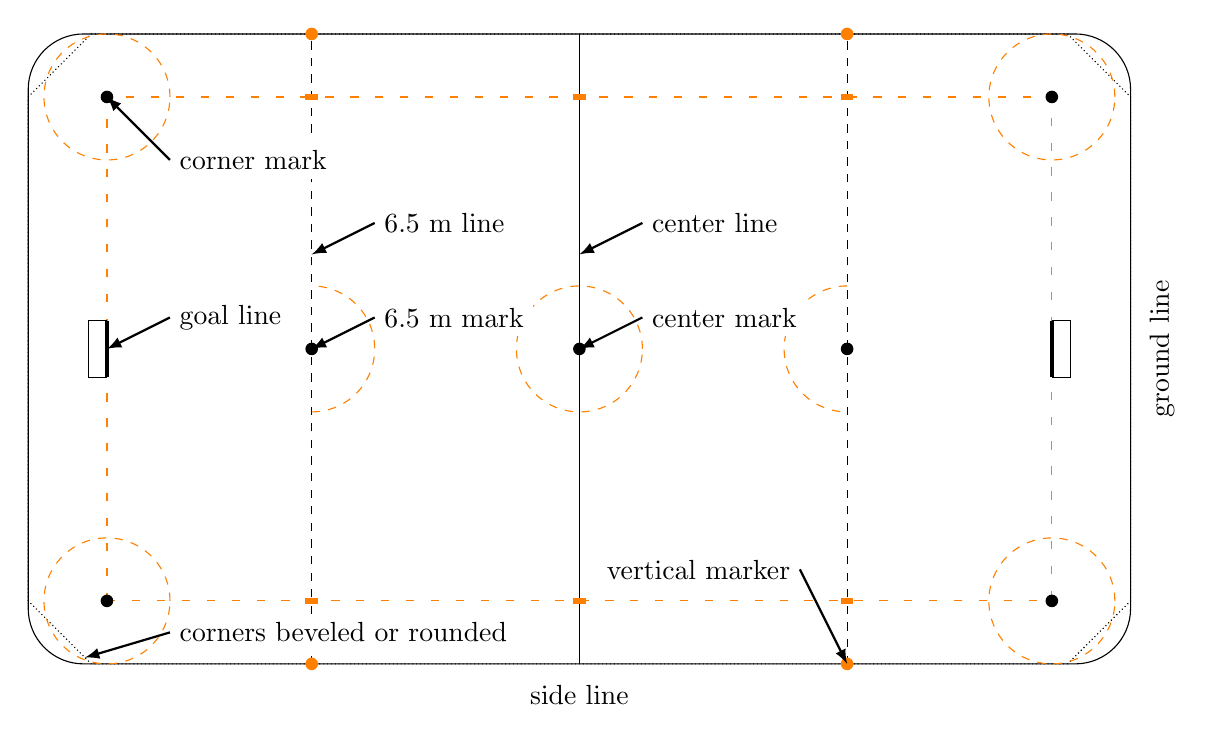
\begin{tikzpicture}[scale=0.4]%(1600,1000)
\usetikzlibrary{calc}
% length:
\dimline[line style = {line width=0.9},]{(0,21)}{(35,21)}{length: 35 - 45 m}
\dimline[line style = {line width=0.9},]{(-1,0)}{(-1,20)}{breadth: 20 - 25 m}
\dimline[line style = {line width=0.9},]{(35-2.5-6.5,15)}{(35-2.5,15)}{6.5 m}
\dimline[label style={above=0.5ex,}, line style = {line width=0.9},]{(32.5,5)}{(35,5)}{2.5 m}
\dimline[label style={above=0.5ex,}, line style = {line width=0.9},]{(28.75,0)}{(28.75,2)}{2 m}

% field:
\draw[rounded corners=20pt] (0,0) rectangle ++(35,20);
\draw[densely dotted] (0,2) -- (0,18) -- (2,20) -- (33,20) -- (35,18) -- (35,2) -- (33,0) -- (2,0) -- (0,2);
\draw[orange, loosely dashed] (2.5,2) -- (2.5,18) -- (32.5,18) -- (32.5,2) -- (2.5,2);
% corner marks:
\fill (2.5,2) circle (0.2);
\draw[orange, dashed] (2.5,2) circle (2);
\fill (2.5,18) circle (0.2);
\draw[orange, dashed] (2.5,18) circle (2);
\fill (35-2.5,18) circle (0.2);
\draw[orange, dashed] (35-2.5,18) circle (2);
\fill (35-2.5,2) circle (0.2);
\draw[orange, dashed] (35-2.5,2) circle (2);
% center line:
\draw[] (17.5,0) -- (17.5,20);
% center mark:
\fill (17.5,10) circle (0.2);
\draw[orange, dashed] (17.5,10) circle (2);
% 6.5 m lines:
\draw[dashed] (2.5+6.5,0) -- (2.5+6.5,20);
\draw[dashed] (35-2.5-6.5,0) -- (35-2.5-6.5,20);
% 6.5 m marks:
\fill (2.5+6.5,10) circle (0.2);
\draw[orange, dashed] (2.5+6.5,8) arc(-90:90:2);
\fill (35-2.5-6.5,10) circle (0.2);
\draw[orange, dashed] (35-2.5-6.5,12) arc(90:270:2);
% goal line:
\draw[line width=0.5mm,] (2.5,9.1) -- (2.5,10.9);
\draw[line width=0.5mm,] (35-2.5,9.1) -- (35-2.5,10.9);

%intersection marks:
%\fill[orange] (2.5+6.5,2) circle (0.2);
%\fill[orange] (2.5+6.5,18) circle (0.2);
%\fill[orange] (17.5,2) circle (0.2);
%\fill[orange] (17.5,18) circle (0.2);
%\fill[orange] (35-2.5-6.5,2) circle (0.2);
%\fill[orange] (35-2.5-6.5,18) circle (0.2);
\drawRectangle{2.5+6.5}{2}{0.4}{0.2}
\drawRectangle{2.5+6.5}{18}{0.4}{0.2}
\drawRectangle{17.5}{2}{0.4}{0.2}
\drawRectangle{17.5}{18}{0.4}{0.2}
\drawRectangle{35-2.5-6.5}{2}{0.4}{0.2}
\drawRectangle{35-2.5-6.5}{18}{0.4}{0.2}

%vertival marks
\fill[orange] (2.5+6.5,0) circle (0.2);
\fill[orange] (2.5+6.5,20) circle (0.2);
\fill[orange] (35-2.5-6.5,0) circle (0.2);
\fill[orange] (35-2.5-6.5,20) circle (0.2);

% goals
\draw (2.5,9.1) -- (1.9,9.1) -- (1.9,10.9) -- (2.5,10.9);
\draw (32.5,9.1) -- (33.1,9.1) -- (33.1,10.9) -- (32.5,10.9);

% labels
\node[right, fill=white] at (4.5,16) (Corner-Mark) {corner mark};
\draw[-latex,thick] (4.5,16) -- (2.5,18);
\node[right] at (4.5,11) (Goal-Line) {goal line};
\draw[-latex,thick] (4.5,11) -- (2.5,10);
\dimline[line style = {line width=0.9},]{(0,5)}{(2.5+6.5,5)}{goal area}
%\node[fill=white] at (4.75,5) (Goal-Area) {goal area};
\node[right, fill=white] at (11,11) (6.5-Mark) {6.5 m mark};
\draw[-latex,thick] (11,11) -- (2.5+6.5,10);
\node[right] at (11,14) (6.5-Line) {6.5 m line};
\draw[-latex,thick] (11,14) -- (2.5+6.5,13);
\node[right, fill=white] at (19.5,11) (Center-Mark) {center mark};
\draw[-latex,thick] (19.5,11) -- (17.5,10);
\node[right] at (19.5,14) (Center-Line) {center line};
\draw[-latex,thick] (19.5,14) -- (17.5,13);
\node[left, fill=white] at (24.5,3) (VerticalMarker) {vertical marker};
\draw[-latex,thick] (24.5,3) -- (26,0);
\node at (17.5,-1) (Side-Line) {side line};
\node[rotate=90] at (36,10) (Ground-Line) {ground line};

\node[right, fill=white] at (4.5,1) {corners beveled or rounded};
\draw[-latex,thick] (4.5,1) -- (1.8,0.2);
\end{tikzpicture}


The field has a length of 35 to 45 meters and a breadth of 20 to 25 meters.
It is surrounded by barriers (boards or walls).
The corners are rounded or beveled.
Any surface outside, or above the barriers, is not considered in the field.

\subsection{Goals}
The goal posts are 2.50\,m in from the ends of the playing field (ground lines), ensuring that the players can go behind them.
The inside dimensions of goal openings are 1.20\,m high and 1.80\,m wide.
The goals must be made in such a way that the ball cannot enter through the rear or sides.
The goals must not have sharp, pointed or protruding parts.

\subsection{Markings}
The center line divides the field into two equal halves, and the center mark is in the middle of the center line.
There are marks in front of each goal at a distance of 6.5\,m.
A 5\,cm wide goal line shall be marked on the ground between the goal posts, with the front edge of the goal line (the side closest to the center mark) in line with the front face of the goal posts.
The corner marks are on the extension of the goal lines, 2\,m in from the boundaries.
The 6.5\,m lines are parallel to the goal lines and run through the 6.5\,m marks.
The 6.5\,m lines shall be vertically marked on the barriers or walls of the playing field.
The goal areas are between the 6.5\,m lines and the ends of the field.

Two meters from each side line, T-markings shall be placed on the center line and the 6.5\,m lines to visually identify the 2\,m infield boundary for free shots.
These T-markings may be connected by dashed lines.
Circles of 2\,m radius may be marked around the center mark, each corner mark and each 6.5\,m mark to visually enforce the minimum distance players must observe during face-offs, free-shots or penalties.

\section{Ball}
A tennis ball that rebounds off concrete greater than 30 percent of the height from which it was dropped is used.

\section{Practice Time}
At a tournament, sufficient practice time and/or warm up time must be offered to the participants.

\section{Penalty Box}
Designated seating for the penalty box must be provided on each half of the field, arranged so that players who are sent off remain separated from their teammates and the opposing team throughout the send-off period.